% =====================================================================
%  paper_revised.tex  --  REVISED version of IConSCEPT 2026 paper #633
%
%  IMPORTANT: the original main.tex was NOT in the repository (the
%  Drone-Detection-1 submodule commit 12c69f7 was never pushed). This file
%  was rebuilt from the submitted PDF (YOLOv8_CBAM_Paper_10.pdf) and then
%  revised. Diff it against your own main.tex before submitting.
%
%  * Text changed in the revision is wrapped in \rev{...} and shown in blue.
%    Set \revisionmarksfalse below to print everything in black.
%  * Every number added in the revision comes from revision/results/*.json;
%    tables are generated by revision/d_fill_tables.py (do not edit by hand).
%  * Lines marked "% TODO(GPU)" need the GPU experiments / trained weights.
%
%  Build:  cd revision && pdflatex paper_revised && pdflatex paper_revised
% =====================================================================
\documentclass[conference]{IEEEtran}
\IEEEoverridecommandlockouts
\usepackage{cite}
\usepackage{amsmath,amssymb,amsfonts}
\usepackage{graphicx}
\usepackage{booktabs}
\usepackage{subcaption}
\usepackage{xcolor}
\usepackage{url}

\newif\ifrevisionmarks
\revisionmarkstrue            % <- set to \revisionmarksfalse for the final camera-ready
\ifrevisionmarks
  \newcommand{\rev}[1]{{\color{blue}#1}}
\else
  \newcommand{\rev}[1]{#1}
\fi

\graphicspath{{figures/}{evidence/paper_pdf_figures/}}

\begin{document}

\title{An Attention-Guided Neck Feature Fusion Framework for Drone Detection Using YOLOv8 and CBAM}

\author{\IEEEauthorblockN{Rohith S, Krithik JY, Avantika R, Thilak Sujan KS, Karthika R*}
\IEEEauthorblockA{Department of Electronics and Communication Engineering\\
Amrita School of Engineering, Coimbatore\\
Amrita Vishwa Vidyapeetham, India\\
*Corresponding author: r\_karthika@cb.amrita.edu}}

\maketitle

% ---------------------------------------------------------------------
\begin{abstract}
Small unmanned aerial vehicles (UAVs) can be challenging to detect in outdoor images, particularly when they appear
at a distance and occupy only a small portion of the frame. Their appearance can also be easily confused with birds,
vegetation, clouds, buildings, and other background elements. To address this challenge, this paper proposes an
attention-guided enhancement of the You Only Look Once (YOLO) detector YOLOv8x by incorporating the Convolutional
Block Attention Module (CBAM) at two selected feature-fusion stages in the path aggregation neck. Specifically,
channel attention followed by spatial attention is introduced after the $40\times40$ and $80\times80$
feature-fusion stages, allowing the network to refine the multi-scale features before they are passed to the
detection head. Rather than making extensive changes to the YOLOv8x backbone, the proposed approach retains the
original feature hierarchy and \rev{adds 64,198 parameters (0.094\%) and 0.0018 GFLOPs}. On the original validation
split, the proposed model reaches a mean average precision of 92.93\% at mAP@0.5 and 57.10\% at mAP@0.5:0.95,
\rev{3.71 and 3.34 percentage points above the reported baseline. We further audit the dataset, find
near-duplicate images shared by the original training and validation sets, and provide a leakage-free,
scene-grouped train/validation/test split together with a fully scripted evaluation protocol.}
The ablation study shows that channel and spatial attention contribute in different but complementary ways.
\end{abstract}

\begin{IEEEkeywords}
drone detection, UAV detection, YOLOv8, CBAM, attention mechanism, object detection, small object detection,
feature fusion
\end{IEEEkeywords}

% ---------------------------------------------------------------------
\section{Introduction}
Unmanned aerial vehicles (UAVs), or drones, are now used well beyond military settings, in tasks such as
infrastructure inspection, precision agriculture, package delivery, mapping, disaster response, and surveillance.
Their low cost and agility, however, also raise security concerns, including intrusion into restricted airspace,
smuggling, covert surveillance, and collision risks near airports. This growth is part of a wider rise of small
autonomous robots, which now extends even to bioinspired microrobots for medical use~\cite{rajagopal2025}.

Spotting low-flying drones in cluttered outdoor scenes is still difficult. Seen from a ground camera, a drone may
cover only $16\times16$ to $32\times32$ pixels of a high-definition frame, so fine details such as propellers, motor
mounts, and the airframe are largely lost after downsampling. Its appearance also changes with viewing angle,
lighting, motion blur, and partial occlusion by trees, poles, or buildings, while clouds, birds, and moving foliage
can produce drone-like patterns that cause false alarms or missed targets.

Preserving information across scales is therefore essential. Feature Pyramid Networks (FPN)~\cite{fpn} and Path
Aggregation Networks (PANet)~\cite{panet} merge features from different resolutions, but this fusion can also carry
background noise into the feature maps and blur the edges of small objects. Attention mechanisms address this by
weighting features according to their channel and spatial importance, and the Convolutional Block Attention Module
(CBAM)~\cite{cbam} does so by applying channel attention followed by spatial attention.

In this work, two CBAM modules are added to the path aggregation neck of YOLOv8x, after the $40\times40$ fusion
stage at Layer~12 and the $80\times80$ fusion stage at Layer~15. These are the points where features from different
scales meet, so refining them here is intended to suppress background clutter and keep the visual cues of drones
before detection.

The main contributions of this work are as follows:
\begin{itemize}
\item We propose YOLOv8-CBAM, an attention-guided architecture for UAV detection in visually complex outdoor
environments.
\item We introduce a targeted neck-level attention strategy by placing two CBAM modules after Layers~12 and~15,
enhancing the fused feature representations while keeping the original YOLOv8x architecture unchanged.
\item We conduct an ablation study comparing the baseline YOLOv8x with channel-only attention, spatial-only
attention, and the complete CBAM configuration\rev{, and provide scripts for placement, attention-type, multi-seed
and state-of-the-art comparisons on a leakage-free split}.
\item \rev{We report measured complexity: CBAM adds 64,198 parameters (+0.094\%) and 0.0018 GFLOPs (+0.0007\%) to
the 68.15\,M-parameter, 258.11-GFLOP detector, and we audit the benchmark for train/validation near-duplicates.}
\end{itemize}

\begin{figure*}[!t]
\centering
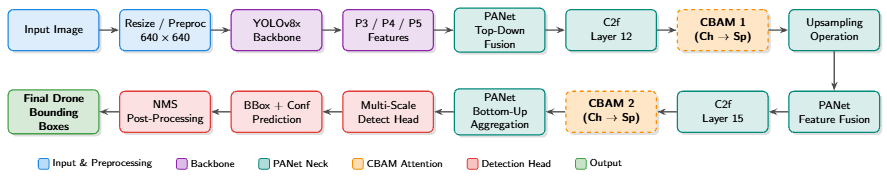
\includegraphics[width=0.9\textwidth]{fig1_pipeline.png}
\caption{End-to-end pipeline of the proposed YOLOv8-CBAM drone detection framework.}
\label{fig:pipeline}
\end{figure*}

% ---------------------------------------------------------------------
\section{Related Work}
\subsection{Deep Learning Object Detection}
Object detectors built on deep learning are usually grouped into two-stage and single-stage designs. Two-stage
methods such as Faster R-CNN~\cite{fasterrcnn} first propose candidate regions and then classify and refine them,
which gives good accuracy but slows down inference. Single-stage methods such as SSD~\cite{ssd} and the YOLO family
predict classes and boxes in a single pass, which makes them better suited to real-time use. YOLOv4~\cite{yolov4}
brought in a CSPNet backbone, PANet feature routing, and mosaic augmentation, while YOLOv7~\cite{yolov7} improved
efficiency through extended efficient layer aggregation. YOLOv8~\cite{ultralytics} then added the C2f block for
better gradient flow and feature reuse, together with an anchor-free decoupled head\rev{; YOLO11 and the
transformer-based RT-DETR~\cite{rtdetr} are used here as additional comparison detectors}.

\subsection{Multi-Scale Representation and Attention}
Small objects are hard to detect because deeper layers gain semantic information at the cost of spatial
resolution. FPN~\cite{fpn} handles this with a top-down path and lateral connections that merge features across
scales, and PANet~\cite{panet} adds a bottom-up path so that low-level spatial detail reaches the deeper layers more
easily. Improved YOLOv5 variants have applied similar ideas to general object detection~\cite{mohankumar2023} and to
finding small defects on cluttered printed circuit boards~\cite{venkatesan2025}.

Attention modules take a different route by weighting features according to how useful they are.
Squeeze-and-Excitation (SE) networks~\cite{senet} learn channel weights from globally pooled features, while
CBAM~\cite{cbam} adds a spatial branch so that the network learns both which channels and which locations matter.
Coordinate Attention~\cite{coordatt} builds position information into channel attention by pooling along each
spatial direction, and CBAM SAUNet~\cite{rajamani2024} showed that combining channel and spatial attention helps with
difficult corner cases in segmentation.

% ---------------------------------------------------------------------
\section{Dataset and Problem Formulation}
\subsection{Dataset Attributes and Annotation}
This study uses the publicly available YOLO Drone Detection Dataset from Kaggle~\cite{kaggle}, which contains 1,359
images of a single class, drone, captured against clear and overcast skies, urban skylines, and dense vegetation.
The original release is split into 1,012 training (74.5\%) and 347 validation (25.5\%) images \rev{with 1,117 and
369 boxes, respectively}. Each drone is labeled with a normalized bounding box
\begin{equation}
b = (x_c, y_c, w, h),
\end{equation}
where $(x_c, y_c)$ is the box center and $w$ and $h$ are its width and height. All images are letterbox-resized to
$640\times640$ pixels so that their aspect ratio is preserved.

As Fig.~\ref{fig:labels} shows, box centers cluster near the middle of the frame and box sizes vary widely.
\rev{Measured after letter-boxing to 640\,px with the COCO thresholds, only 13 of the 1,117 training boxes (1.2\%)
and 25 of the 369 validation boxes (6.8\%) are small ($<32^2$ pixels); 81.8\% of the validation boxes are large
($\geq96^2$). The benchmark is therefore dominated by close-range drones, which limits how strongly it can test
small-object detection (Section~\ref{sec:limitations}).}

\rev{\textit{Provenance and near-duplicate audit.} The images come from several sources whose file names identify
them: web photographs (\texttt{pic\_*}, numeric names) and frames sampled from videos (\texttt{foto*},
\texttt{yoto*}, \texttt{scene*}). We hashed every image with a 64-bit perceptual hash (pHash) and compared all
train--validation pairs (Table~\ref{tab:split}). In the original split, 33 of the 347 validation images (9.5\%) have
a near-duplicate (Hamming distance $\leq4$) in the training set, 30 of them identical pictures stored under
different names, and 48 (13.8\%) have a same-scene match ($\leq10$). We therefore built a \emph{scene-grouped}
split: images linked by a pHash distance $\leq10$ or by neighbouring frame numbers ($<100$ apart) of the same video
source are merged into groups, and whole groups are assigned, per source family, to train/validation/test in a
70/15/15 ratio. The result (975/197/187 images) has no cross-split pair within 10 bits. Model selection uses only
the validation part; the test part is evaluated once.}

\begin{figure}[!t]
\centering
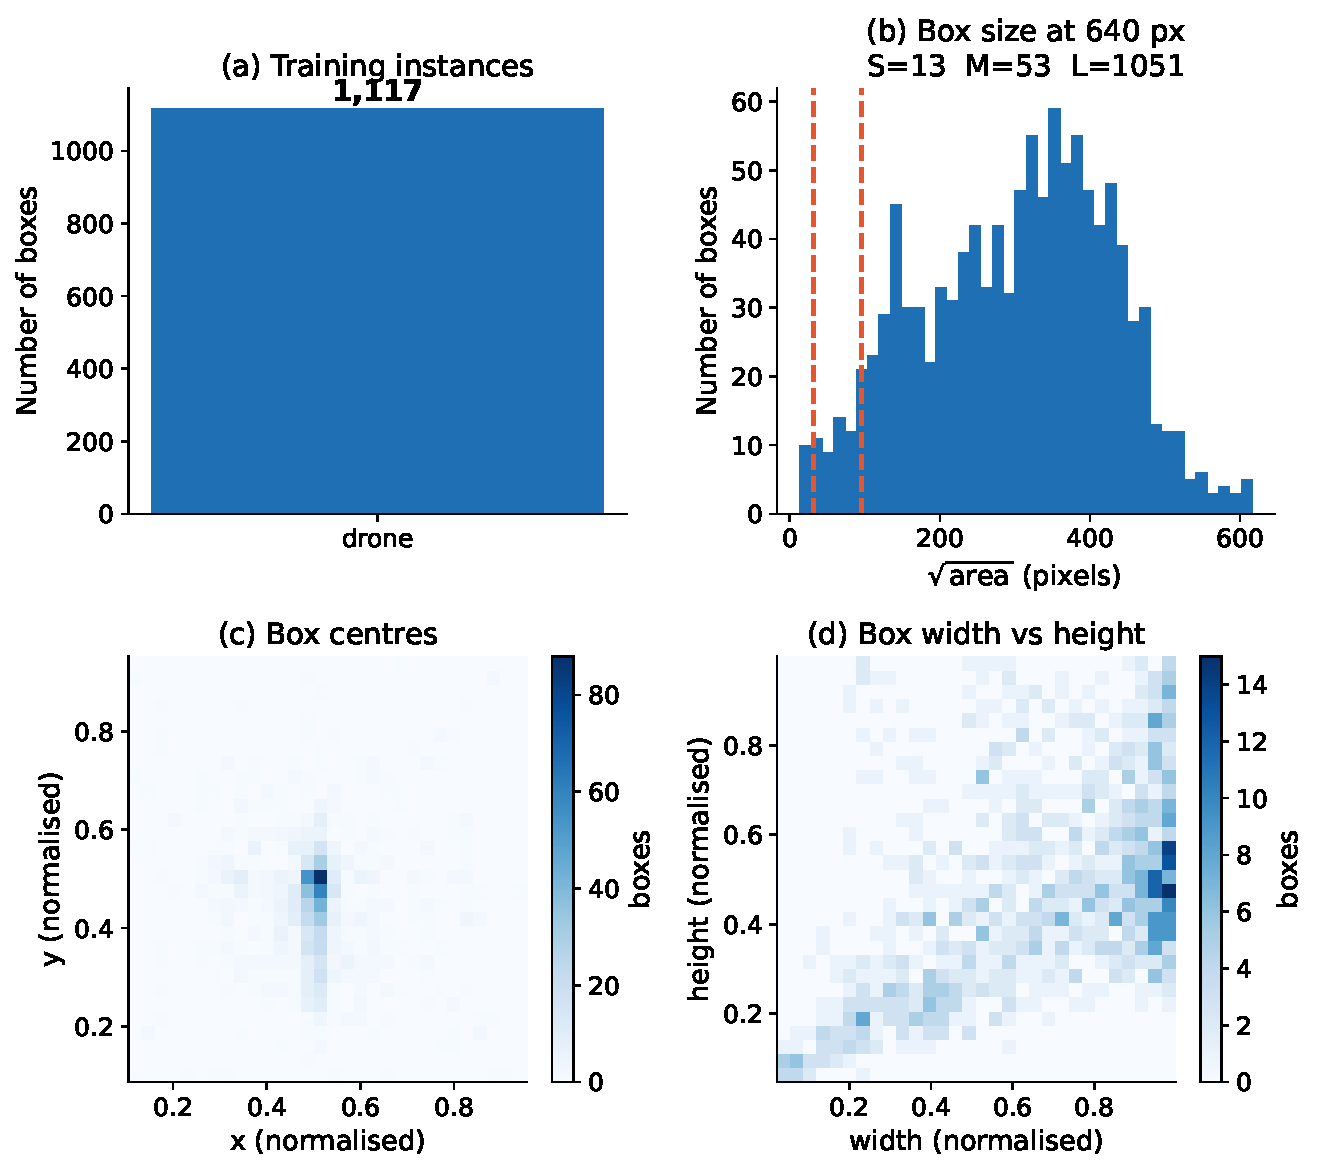
\includegraphics[width=\columnwidth]{fig2_label_statistics.pdf}
\caption{Statistics of the training annotations: (a) number of drone instances, (b) box size after letter-boxing to
640\,px with the COCO small/large borders (dashed), (c) distribution of normalized box centers, and (d) joint
distribution of normalized box width and height.}
\label{fig:labels}
\end{figure}

\subsection{Formal Detection Objective}
The detector is trained by minimizing a combined loss function:
\begin{equation}
L_{total} = \lambda_{box} L_{CIoU} + \lambda_{cls} L_{BCE} + \lambda_{dfl} L_{DFL}.
\end{equation}
Here, Complete Intersection over Union (CIoU) loss is used for bounding-box localization, Binary Cross-Entropy (BCE)
loss handles classification, and Distribution Focal Loss (DFL) helps improve localization\rev{; the Ultralytics
defaults $\lambda_{box}=7.5$, $\lambda_{cls}=0.5$, $\lambda_{dfl}=1.5$ are used}.

% ---------------------------------------------------------------------
\section{Proposed YOLOv8-CBAM Framework}
\subsection{Overall Architectural Pipeline}
As shown in Fig.~\ref{fig:pipeline}, YOLOv8-CBAM keeps the standard YOLOv8x backbone and decoupled anchor-free
detection head, and changes only the path aggregation neck. Two CBAM modules are placed after Layer~12 and Layer~15,
where the $40\times40$ and $80\times80$ features are fused, so that the combined features are refined before they pass
through the bottom-up pathway to the detection head and non-maximum suppression.

\subsection{Backbone and Multi-Scale Feature Hierarchy}
YOLOv8x is used as the base network. Its backbone is built using modified CSPNet blocks called C2f. As the input
passes through the backbone, it is progressively downsampled by factors of 8, 16, and 32, producing three feature
pyramid stages \rev{(channel counts from a tensor-shape trace, Table~\ref{tab:stages})}:
\begin{itemize}
\item P3 ($80\times80$, 320 channels): high-resolution features with fine spatial details.
\item P4 ($40\times40$, 640 channels): medium-resolution features that balance spatial information with semantic
context.
\item P5 ($20\times20$, 640 channels): lower-resolution, deeper features with wider receptive fields through the
Spatial Pyramid Pooling-Fast (SPPF) module.
\end{itemize}

\begin{table}[!t]
\centering
\caption{Principal feature stages of YOLOv8x for a $640\times640$ input (measured by a tensor-shape trace).}
\label{tab:stages}
\setlength{\tabcolsep}{3pt}
\begin{tabular}{clccl}
\toprule
Layer & Module & Channels & Resolution & Role \\
\midrule
0 & Conv ($k{=}3,s{=}2$) & 80 & $320\times320$ & Low-level stem \\
1 & Conv ($k{=}3,s{=}2$) & 160 & $160\times160$ & Downsampling \\
2 & C2f ($n{=}3$) & 160 & $160\times160$ & Feature extraction \\
3 & Conv ($k{=}3,s{=}2$) & 320 & $80\times80$ & Downsampling \\
4 & C2f ($n{=}6$) & 320 & $80\times80$ & P3 multi-scale feature \\
5 & Conv ($k{=}3,s{=}2$) & 640 & $40\times40$ & Downsampling \\
6 & C2f ($n{=}6$) & 640 & $40\times40$ & P4 multi-scale feature \\
7 & Conv ($k{=}3,s{=}2$) & 640 & $20\times20$ & Downsampling \\
8 & C2f ($n{=}3$) & 640 & $20\times20$ & Deep context extraction \\
9 & SPPF ($k{=}5$) & 640 & $20\times20$ & P5 multi-scale feature \\
12 & C2f & 640 & $40\times40$ & Neck fusion / CBAM-1 \\
15 & C2f & 320 & $80\times80$ & Neck fusion / CBAM-2 \\
22 & Detect head & Multi & Multi & Decoupled detection \\
\bottomrule
\end{tabular}
\end{table}


\subsection{CBAM Formulation}
The internal operation of the CBAM module is illustrated in Fig.~\ref{fig:cbam}. For an intermediate feature tensor
$F\in\mathbb{R}^{C\times H\times W}$, CBAM applies channel attention followed by spatial attention. The channel
attention map $M_c\in\mathbb{R}^{C\times1\times1}$ is obtained by applying average and max pooling across the
spatial dimensions. These pooled features are passed through a shared multilayer perceptron (MLP) with a reduction
ratio of $r=16$\rev{, a ReLU activation $\delta$ between its two layers, and no bias terms}, and the results are
combined and passed through a sigmoid function $\sigma$:
\begin{equation}
M_c(F) = \sigma\Big(W_1\,\rev{\delta}\big(W_0(F^c_{avg})\big) + W_1\,\rev{\delta}\big(W_0(F^c_{max})\big)\Big),
\end{equation}
where $W_0\in\mathbb{R}^{C/r\times C}$ and $W_1\in\mathbb{R}^{C\times C/r}$ are the shared MLP weights. The resulting
channel attention is applied to the input feature map through element-wise multiplication:
\begin{equation}
F' = M_c(F)\otimes F.
\end{equation}
Next, the spatial attention module applies average and max pooling along the channel dimension, concatenates the
two maps, and processes them using a $7\times7$ convolution followed by a sigmoid function:
\begin{equation}
M_s(F') = \sigma\big(f^{7\times7}([\mathrm{AvgPool}_c(F'); \mathrm{MaxPool}_c(F')])\big).
\end{equation}
The spatial attention map is applied to the refined feature map:
\begin{equation}
F'' = M_s(F')\otimes F'.
\end{equation}
\rev{Finally, the CBAM output is blended with its input through a learnable scalar gate $\gamma$ that is initialized
to zero,
\begin{equation}
Y = F + \gamma\,(F'' - F),
\end{equation}
so that at the start of fine-tuning the network reproduces the pretrained YOLOv8x exactly and learns how much
attention to apply.} % VERIFY against your cbam.py: the gate is inferred from scratch/verify_cbam_refactor.py

\begin{figure}[!t]
\centering
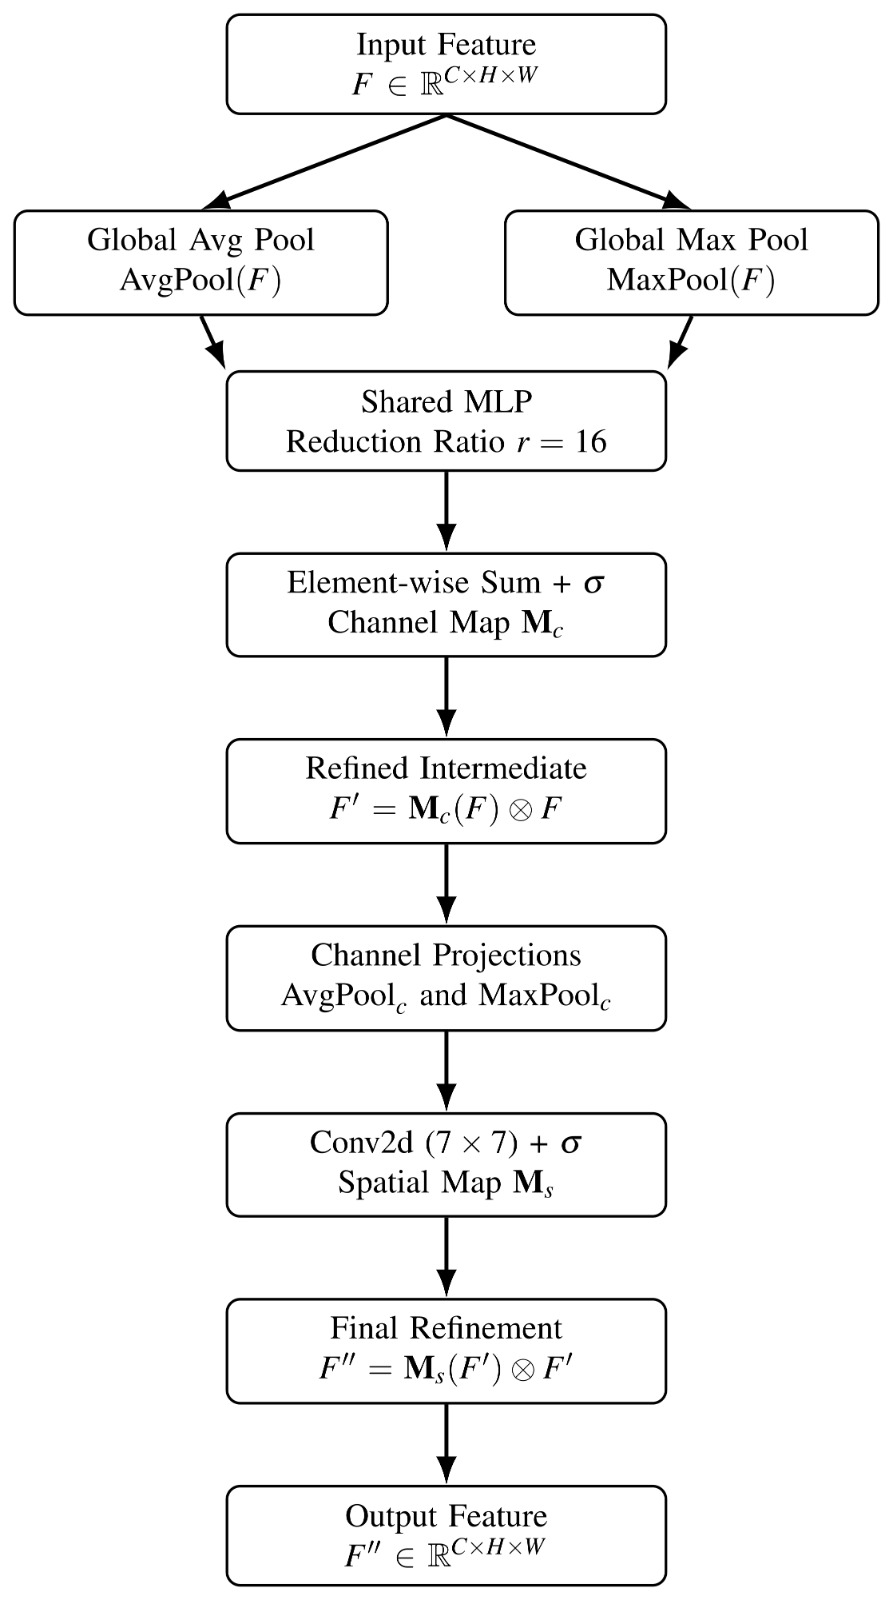
\includegraphics[width=0.75\columnwidth]{fig3_cbam.png}
\caption{CBAM sequential channel-then-spatial attention workflow.}
\label{fig:cbam}
\end{figure}

\subsection{Targeted Attention Placement}
Instead of adding attention modules throughout the network, we place two CBAM modules at feature-fusion points in
the neck:
\begin{itemize}
\item CBAM-1 (Layer~12): placed after the C2f Layer~12 and operating on a \rev{$640\times40\times40$} feature map,
where upsampled P5 features are combined with P4 features.
\item CBAM-2 (Layer~15): placed after the C2f Layer~15 and operating on a \rev{$320\times80\times80$} feature map,
where top-down semantic information is combined with high-resolution P3 features before the bottom-up
aggregation stage.
\end{itemize}

\subsection{\rev{Attention Integration and Training}}
\rev{The attention modules are attached by \emph{module wrapping}: the C2f modules at indices 12 and 15 of the
Ultralytics layer list are replaced by a wrapper that first runs the original C2f block and then the gated CBAM of
Eq.~(7). The wrapper copies the layer's routing attributes, so the rest of the network is unchanged, and the same
code switches between full CBAM, channel-only, spatial-only and baseline execution. The wrapper is inserted
\emph{after} the COCO-pretrained YOLOv8x weights are loaded, which preserves the pretrained initialization. The
original weights are \emph{not} frozen: all parameters (except the fixed DFL projection) are fine-tuned jointly with
CBAM. We verified that (i) all CBAM tensors, including both gates $\gamma$, are registered in the optimizer,
(ii) the wrapped modules and gate values are stored in and restored from Ultralytics checkpoints, and (iii) the model
exports to ONNX (opset~17) with a maximum deviation of $9.7\times10^{-4}$ from PyTorch. Because stock Ultralytics
rebuilds the network from its YAML file at the start of training, the wrapping is applied inside a custom trainer's
\texttt{get\_model()}.}

% ---------------------------------------------------------------------
\section{Implementation and Training Setup}
\subsection{Training Protocol and Hyperparameters}
The experiments were conducted using PyTorch with automatic mixed precision, with the YOLOv8x network initialized
from COCO-pretrained weights. The settings are summarized in Table~\ref{tab:hyper}. \rev{The Ultralytics default
augmentation was used: mosaic (probability 1.0, disabled for the last 10 epochs), horizontal flip (0.5), random
scaling ($\pm50\%$), translation ($\pm10\%$) and HSV perturbation (0.015, 0.7, 0.4), with a 3-epoch warm-up and a
linear learning-rate decay to $0.01\eta_0$. For every configuration the checkpoint with the best Ultralytics fitness
($0.1\,\mathrm{mAP@0.5}+0.9\,\mathrm{mAP@0.5{:}0.95}$) on the validation data is reported.}

\begin{table}[!t]
\centering
\caption{Hyperparameter and Training Specifications}
\label{tab:hyper}
\begin{tabular}{ll}
\toprule
Hyperparameter & Setting \\
\midrule
Base model & YOLOv8x (COCO-pretrained) \\
Input size & $640\times640$ (letterbox) \\
Training epochs & 32 \\
Batch size & 16 \\
Optimizer & SGD, momentum 0.937\rev{$^{\ast}$} \\
Weight decay & 0.0005 \\
Initial learning rate $\eta_0$ & 0.01\rev{$^{\ast}$} \\
Channel reduction ratio $r$ & 16 \\
Spatial kernel & $7\times7$ \\
Classes & 1 (drone) \\
\rev{Checkpoint} & \rev{best fitness on validation} \\
\rev{Seed} & \rev{0 (0, 1, 2 in Table~\ref{tab:seeds})} \\
\bottomrule
\end{tabular}\\[2pt]
\footnotesize{\rev{$^{\ast}$The M1 baseline of Table~\ref{tab:ablation} was trained with Ultralytics 8.0.141 and
\texttt{optimizer=auto}, which selected AdamW ($\eta_0=0.002$, momentum 0.9).}}
\end{table}

\subsection{\rev{Evaluation Protocol and Metrics}}
The detection performance was evaluated using Precision (P), Recall (R), Average Precision (AP), mAP@0.5, and
mAP@0.5:0.95. The AP is the area under the precision--recall curve; mAP@0.5 uses an IoU threshold of 0.5, and
mAP@0.5:0.95 averages over IoU thresholds from 0.5 to 0.95. \rev{All metrics are computed with the Ultralytics
validator using a confidence threshold of 0.001, class-aware NMS at IoU 0.7 and at most 300 detections per image.
P and R are reported at the confidence that maximizes F1. The confusion matrix is drawn at a confidence of 0.25 with
an IoU match threshold of 0.45, so its P/R differ from the tabulated max-F1 values. The baseline M1 used
Ultralytics 8.0.141; the scripted revision experiments use Ultralytics 8.4.201 with PyTorch 2.15.
% TODO: state the Ultralytics version of your modified fork used for M2--M4 (not recoverable from the repository).
GFLOPs are reported as $2\times$ multiply--accumulate operations, profiled with thop directly at $640\times640$;
AP by object size uses pycocotools with the COCO area thresholds applied to boxes rescaled to the 640\,px frame.}

% ---------------------------------------------------------------------
\section{Experimental Results and Analysis}
\subsection{Main Benchmark Comparison}
Table~\ref{tab:ablation} compares the baseline YOLOv8x (M1) with the proposed YOLOv8-CBAM (M4) on the original
validation split; its last row lists the gain over the baseline. The proposed model improves all four metrics, with
Precision rising by 4.48 and Recall by 4.85 \rev{percentage points (pp)}. \rev{Because M1 was trained in a separate
run with a different optimizer and because of the near-duplicates found in the original split, these numbers should
be read together with the matched, leakage-free comparison in Tables~\ref{tab:placement}--\ref{tab:sota}.}

\begin{table*}[!t]
\centering
\caption{Ablation of attention configurations on the original validation split (347 images). Params and GFLOPs are
measured for the 1-class model ($640\times640$, GFLOPs $=2\times$MACs, thop); accuracy values are those of the submitted
version. Gains are in percentage points (pp).}
\label{tab:ablation}
\begin{tabular}{lrrcccc}
\toprule
Configuration & Params & GFLOPs & P (\%) & R (\%) & mAP@0.5 (\%) & mAP@0.5:0.95 (\%) \\
\midrule
M1: Baseline$^{\dagger}$ & 68,153,571 & 258.1123 & 86.82 & 83.90 & 89.22 & 53.76 \\
M2: Channel-only & 68,217,573 & 258.1126 & 88.54 & 85.12 & 90.71 & 54.92 \\
M3: Spatial-only & 68,153,769 & 258.1139 & 89.15 & 86.40 & 91.25 & 55.43 \\
M4: YOLOv8x-CBAM & 68,217,769 & 258.1141 & 91.30 & 88.75 & 92.93 & 57.10 \\
\midrule
Gain (M4$-$M1) & +64,198 & +0.0018 & +4.48 pp & +4.85 pp & +3.71 pp & +3.34 pp \\
\bottomrule
\end{tabular}\\[2pt]
\footnotesize{$^{\dagger}$M1 is the final epoch of a separate run made with Ultralytics 8.0.141 and \texttt{optimizer=auto}
(AdamW, $\eta_0=0.002$), whereas the ablation script used for M2--M4 specifies SGD ($\eta_0=0.01$); no raw outputs of
M2--M4 were retained. The matched-protocol comparison on a leakage-free split is Table~\ref{tab:seeds}.}
\end{table*}

\begin{table}[!t]
\centering
\caption{Near-duplicate audit of the original split (pHash, Hamming $\leq4$ / $\leq10$ bits) and the new
scene-grouped split used for all retraining.}
\label{tab:split}
\setlength{\tabcolsep}{4pt}
\begin{tabular}{lccc}
\toprule
\multicolumn{4}{l}{\textit{Original split (1,012 train / 347 val)}} \\
Val images with near-duplicate in train & \multicolumn{3}{c}{33 (9.5\%)} \\
Val images with same-scene match in train & \multicolumn{3}{c}{48 (13.8\%)} \\
\midrule
\textit{Scene-grouped split} & Train & Val & Test \\
Images & 975 & 197 & 187 \\
Boxes & 1042 & 235 & 209 \\
Cross-split pairs $\leq10$ bits & \multicolumn{3}{c}{0} \\
\bottomrule
\end{tabular}
\end{table}


\subsection{Ablation Study on Attention Components}
To separate the effect of each attention branch, we compare four settings: the plain baseline (M1), channel
attention only (M2), spatial attention only (M3), and full CBAM (M4), each applied after Layers~12 and~15.
Table~\ref{tab:ablation} shows that both single branches improve on the baseline, with the spatial branch gaining a
little more than the channel branch, while the full CBAM gives the best results on every metric.

\rev{\textit{Placement, attention type and repeatability.} Table~\ref{tab:placement} compares CBAM at Layer~12 only,
at Layer~15 only and at both, as well as SE and Coordinate Attention at Layers~12+15, under identical settings on
the scene-grouped split. Table~\ref{tab:seeds} reports the baseline and CBAM over three seeds, and
Table~\ref{tab:sota} compares YOLOv8x-CBAM with YOLOv5x, YOLO11x and RT-DETR-X trained under the same protocol.}
% TODO(GPU): after running c11/c12/c13 and d_fill_tables.py, add 2-3 sentences interpreting these tables,
%            e.g. whether the CBAM gain exceeds the seed standard deviation.

\begin{table}[!t]
\centering
\caption{Placement and attention-type ablation on the test split (seed 0). Added parameters are measured. Cells marked ``--'' require trained checkpoints / a GPU and were not run in this revision.}
\label{tab:placement}
\setlength{\tabcolsep}{4pt}
\begin{tabular}{lccc}
\toprule
Configuration & Added params & mAP@0.5 & mAP@0.5:0.95 \\
\midrule
None (baseline) & 0 & -- & -- \\
CBAM @ L12 & -- & -- & -- \\
CBAM @ L15 & -- & -- & -- \\
CBAM @ L12+L15 & +64,198 & -- & -- \\
SE @ L12+L15 & +65,022 & -- & -- \\
CoordAtt @ L12+L15 & +50,012 & -- & -- \\
\bottomrule
\end{tabular}
\end{table}

\begin{table}[!t]
\centering
\caption{Test-split results over three seeds (mean $\pm$ sample std, \%). Cells marked ``--'' require trained checkpoints / a GPU and were not run in this revision.}
\label{tab:seeds}
\setlength{\tabcolsep}{3pt}
\begin{tabular}{lcccc}
\toprule
Model & P & R & mAP@0.5 & mAP@0.5:0.95 \\
\midrule
YOLOv8x & -- & -- & -- & -- \\
YOLOv8x-CBAM & -- & -- & -- & -- \\
\bottomrule
\end{tabular}
\end{table}

\begin{table*}[!t]
\centering
\caption{Comparison with state-of-the-art detectors on the held-out test split of the scene-grouped split
(same epochs, input size, batch size and augmentation; seed 0). Cells marked ``--'' require trained checkpoints / a GPU and were not run in this revision.}
\label{tab:sota}
\begin{tabular}{lccccccc}
\toprule
Model & Params (M) & GFLOPs & FPS & P (\%) & R (\%) & mAP@0.5 (\%) & mAP@0.5:0.95 (\%) \\
\midrule
YOLOv5x (u) & -- & -- & -- & -- & -- & -- & -- \\
YOLO11x & -- & -- & -- & -- & -- & -- & -- \\
RT-DETR-X & -- & -- & -- & -- & -- & -- & -- \\
YOLOv8x & -- & -- & -- & -- & -- & -- & -- \\
YOLOv8x-CBAM (ours) & -- & -- & -- & -- & -- & -- & -- \\
\bottomrule
\end{tabular}
\end{table*}


\subsection{Computational Complexity Analysis}
\rev{The two CBAM modules add exactly 64,198 parameters: 51,299 at Layer~12 ($2\cdot640\cdot40$ MLP weights, 98
convolution weights and one gate) and 12,899 at Layer~15, raising the 1-class YOLOv8x from 68,153,571 to 68,217,769
parameters (+0.094\%). Profiled directly at $640\times640$, the cost rises from 258.1123 to 258.1141 GFLOPs
(+0.0018 GFLOPs, +0.0007\%); fvcore gives the same increment. The element-wise operations of the attention
(pooling, sigmoid gating and blending), which these profilers do not count, add a further 0.028 GFLOPs.
The profile reported by Ultralytics' \texttt{model.info()} (+0.10 GFLOPs) is an artifact of extrapolating from a
$32\times32$ proxy image: the cost of the channel MLP does not grow with image size but is multiplied by
$(640/32)^2$.}

\rev{A small arithmetic overhead does not guarantee a negligible runtime overhead, so we also timed the network
(Table~\ref{tab:runtime}). On a 4-thread CPU (FP32), the median latency is 604.59\,ms for the baseline and
606.91\,ms for YOLOv8-CBAM; the median paired difference, +7.67\,ms (+1.27\%), is well below the run-to-run
standard deviation of about 50--58\,ms.} % TODO(GPU): add the FP16 GPU latency, FPS and peak memory (b8_latency.py).

\begin{table}[!t]
\centering
\caption{Measured complexity and runtime (batch 1, $640\times640$, network forward only, Conv+BN fused, median of
interleaved runs).}
\label{tab:runtime}
\setlength{\tabcolsep}{3pt}
\begin{tabular}{llcccc}
\toprule
Model & Device & Prec. & ms/img & FPS & Peak mem (MB) \\
\midrule
Baseline & CPU, 4 thr. & FP32 & 604.59 & 1.65 & n/a \\
CBAM & CPU, 4 thr. & FP32 & 606.91 & 1.65 & n/a \\
\midrule
\multicolumn{6}{l}{Params added by CBAM: +64,198 (+0.094\%)} \\
\multicolumn{6}{l}{GFLOPs added by CBAM: +0.0018 (+0.0007\%)} \\
\bottomrule
\end{tabular}
\end{table}


\begin{figure*}[!t]
\centering
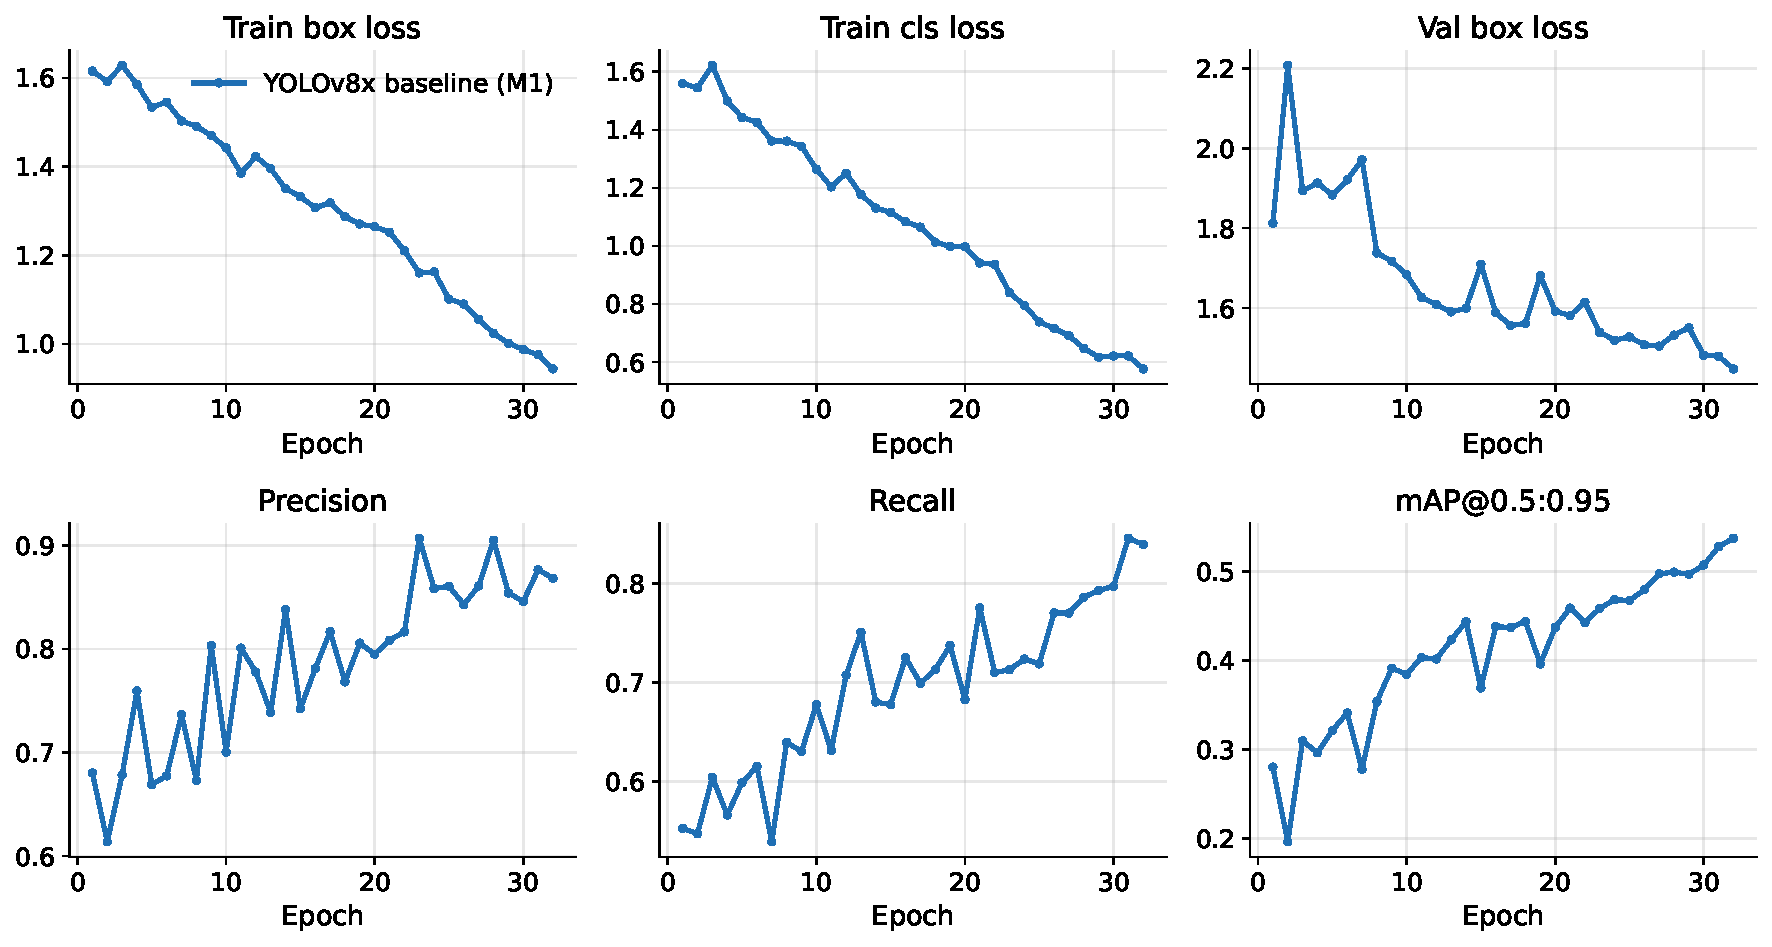
\includegraphics[width=0.85\textwidth]{fig4_training_curves.pdf}
\caption{\rev{Training losses and validation metrics of the baseline YOLOv8x (M1) over its 32 training epochs.}}
% TODO(GPU): add the YOLOv8x-CBAM curve: CBAM_WEIGHTS=<run>/weights/best.pt python d_make_figures.py
\label{fig:curves}
\end{figure*}

% ---------------------------------------------------------------------
\section{Visual and Qualitative Analysis}
\subsection{Training Convergence Dynamics}
Fig.~\ref{fig:curves} illustrates the training convergence \rev{of the baseline over 32 epochs}. The loss curves
decrease steadily, and precision, recall and mAP@0.5:0.95 increase over training; \rev{validation mAP@0.5:0.95 is
still rising at the last epoch (0.528 to 0.538), so a longer schedule may further improve the models.}

\subsection{Confusion Matrix and PR Curves}
\rev{Fig.~\ref{fig:cm} shows the confusion matrix and the precision--recall curve of the \emph{baseline} on the
original validation split. At the confusion-matrix operating point (confidence 0.25, IoU match 0.45) the model finds
320 of the 369 drones and produces 48 false positives, i.e. P = 86.96\% and R = 86.72\%; these differ from
Table~\ref{tab:ablation}, which reports P/R at the max-F1 confidence. Because the validation set contains no
drone-free images, the 48 false positives are spurious boxes on images that do contain a drone; the matrix does not
measure rejection of empty scenes.}
% TODO(GPU): regenerate Fig. 5 for YOLOv8x-CBAM: CBAM_WEIGHTS=<best.pt> python d_make_figures.py

\begin{figure}[!t]
\centering
\begin{subfigure}{0.49\columnwidth}\centering
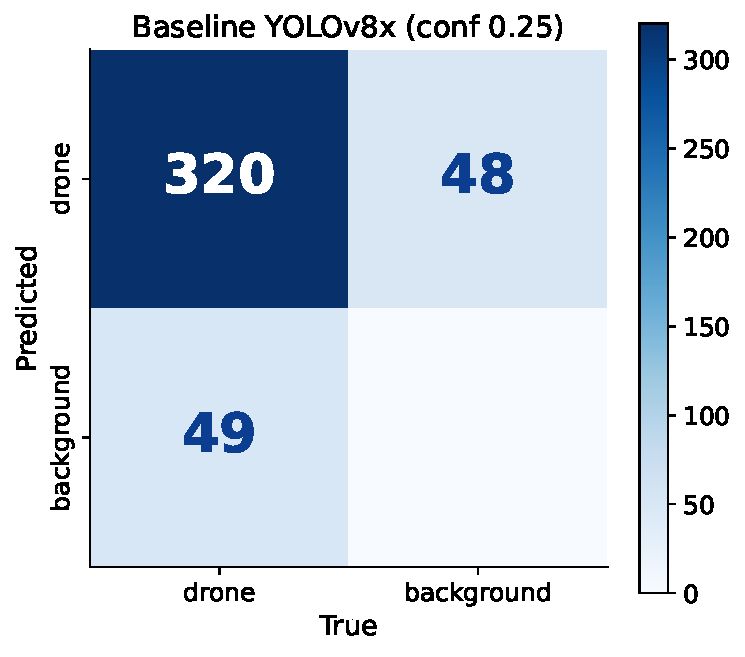
\includegraphics[width=\linewidth]{fig5a_confusion_matrix.pdf}\caption{Confusion matrix}\end{subfigure}\hfill
\begin{subfigure}{0.49\columnwidth}\centering
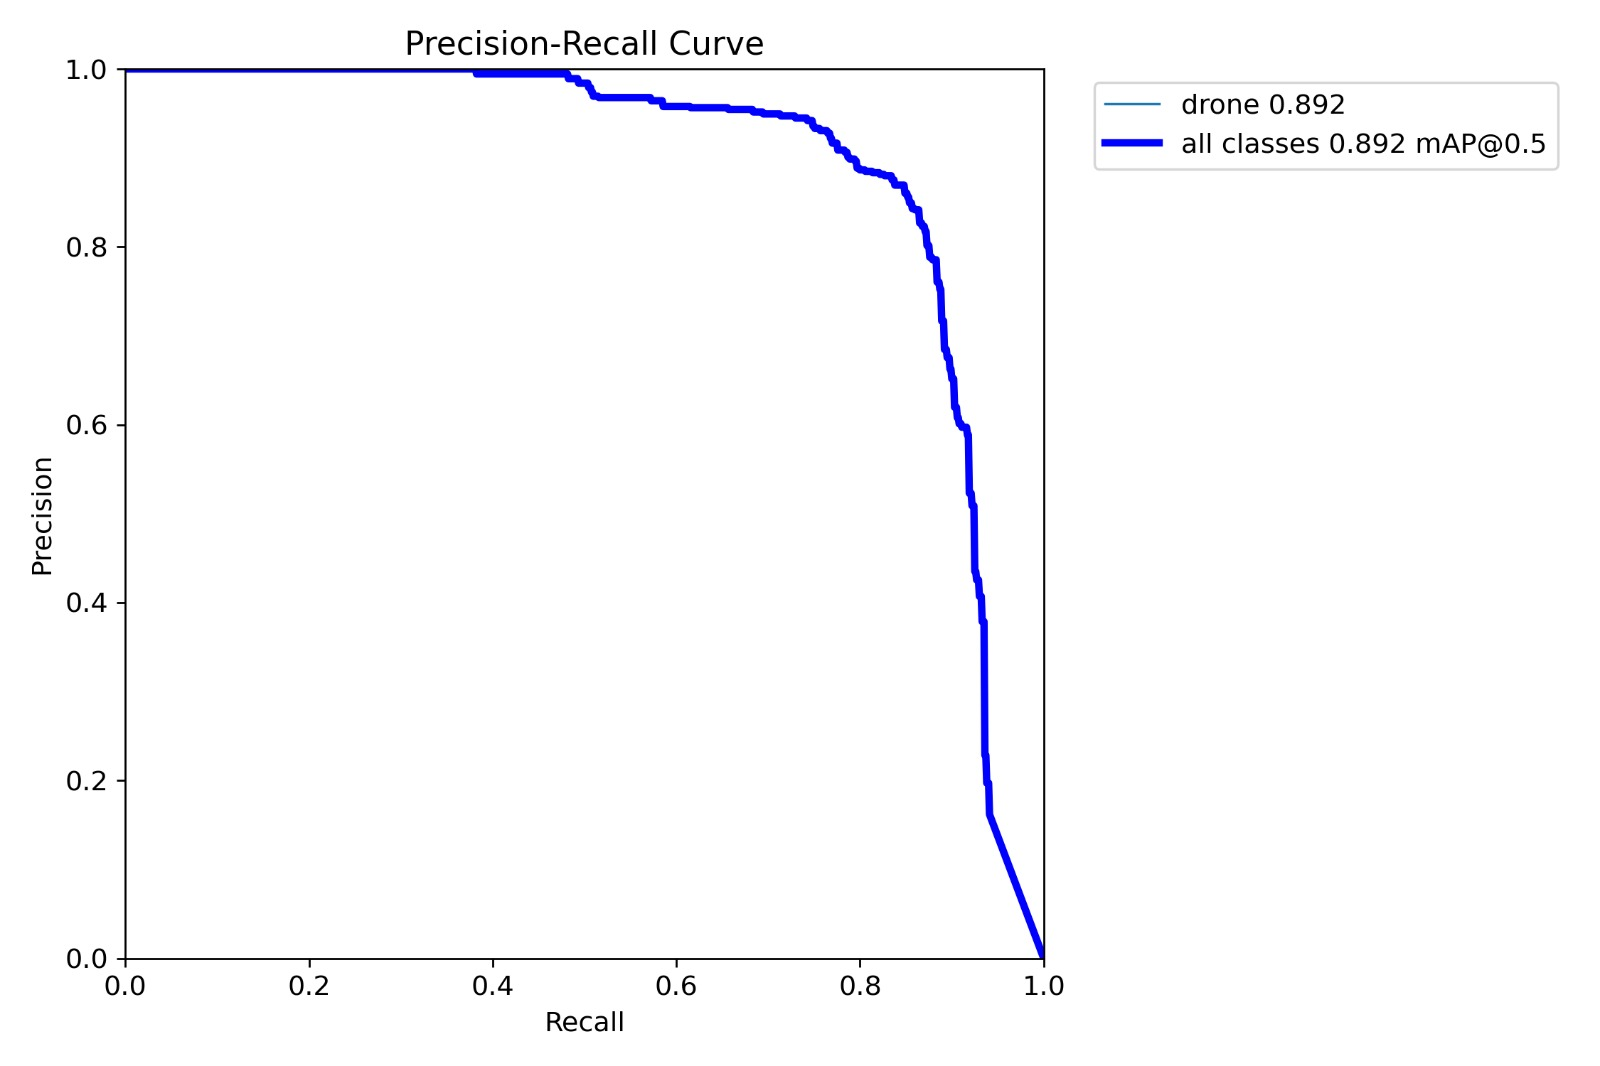
\includegraphics[width=\linewidth]{fig5b_pr_curve.png}\caption{Precision--Recall curve}\end{subfigure}
\caption{\rev{Validation results of the baseline YOLOv8x (M1): (a) confusion matrix at confidence 0.25 and
(b) precision--recall curve (mAP@0.5 = 0.892).}}
\label{fig:cm}
\end{figure}

\subsection{Qualitative Detection Performance}
Fig.~\ref{fig:qual}(a) shows a representative detection produced by YOLOv8-CBAM for a close-range quadcopter
captured against a clear sky, with out-of-focus palm foliage in the background. The model detects the drone with a
confidence score of 0.79, and the textured vegetation behind the airframe does not trigger additional detections.
The predicted box covers the main airframe and all four rotors but excludes part of the lower gimbal camera and the
landing skids, showing that box boundaries can be imprecise for large near-field targets even when the detection is
correct, consistent with the gap between mAP@0.5 and mAP@0.5:0.95.

\subsection{Detection in Cluttered Ground-Level Scenes}
Fig.~\ref{fig:qual}(b) shows a ground-level scene in which a multirotor drone with extended landing gear hovers at
medium range above a dense tree line, with several people and pieces of equipment in the foreground. Despite the
low evening illumination, the model localizes the drone with a tight bounding box, and no detections are produced
on the people, trees, or ground equipment. The confidence of 0.62 is lower than in Fig.~\ref{fig:qual}(a), as the
drone occupies a smaller portion of the frame and its thin arms and legs provide fewer distinctive cues.

\begin{figure*}[!t]
\centering
\begin{subfigure}{0.48\textwidth}\centering
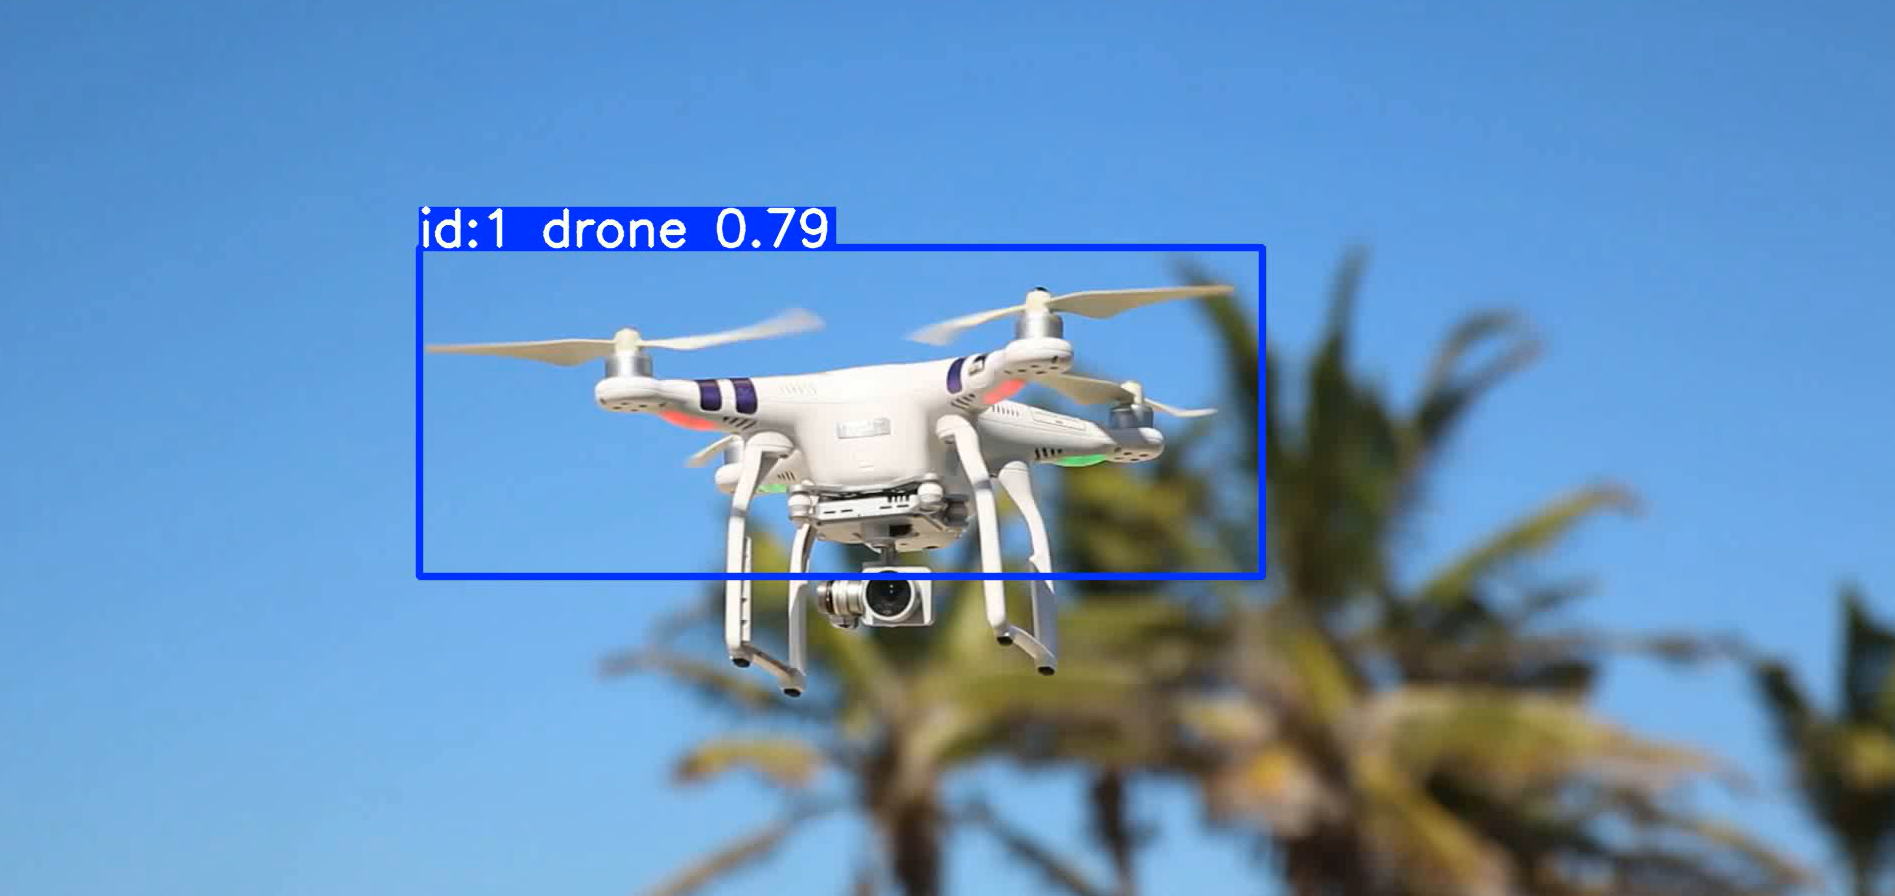
\includegraphics[width=\linewidth]{fig6a.png}\caption{Close-range quadcopter against a clear sky}\end{subfigure}\hfill
\begin{subfigure}{0.48\textwidth}\centering
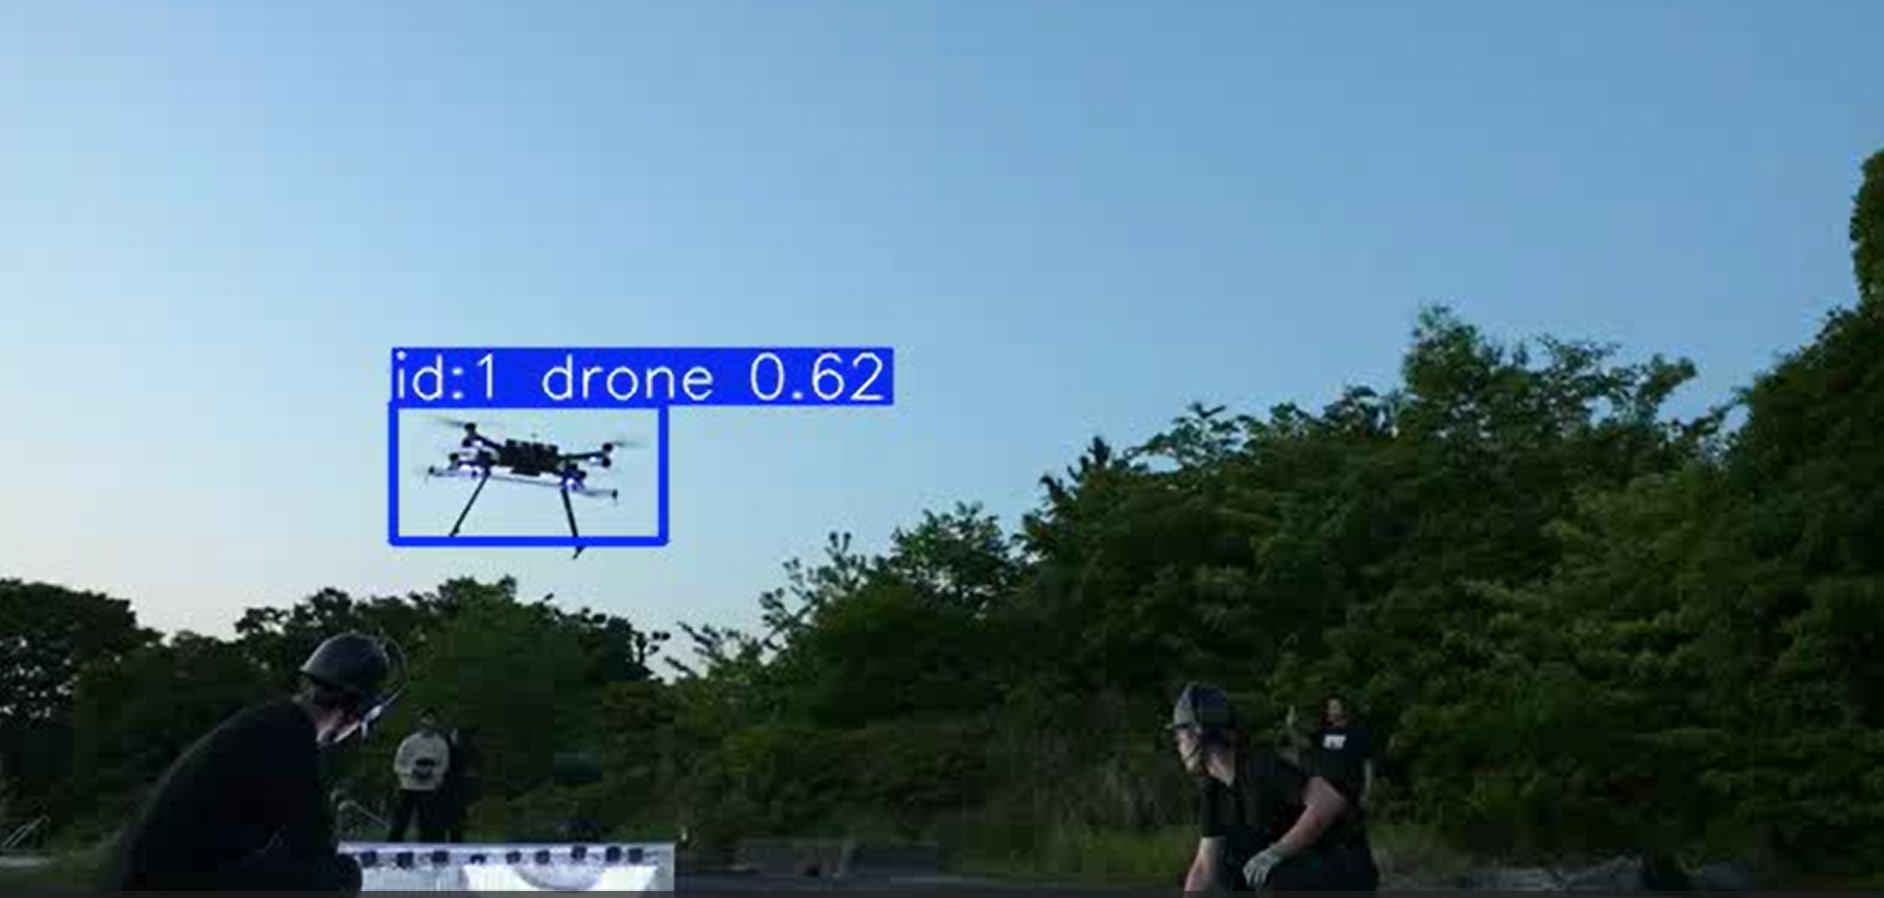
\includegraphics[width=\linewidth]{fig6b.png}\caption{Multirotor drone above a tree line}\end{subfigure}
\caption{Detection results of YOLOv8-CBAM. \rev{The frames were taken from a video-tracking demonstration; the
leading number in each label is the tracker ID and is not part of the detection method.}}
% TODO(GPU): replace with predict() outputs without track IDs: CBAM_WEIGHTS=<best.pt> python d_make_figures.py
\label{fig:qual}
\end{figure*}

\rev{\textit{Failure cases.} Missed or poorly localized drones occur mainly under severe motion blur, at extreme
distances where the drone occupies fewer than $8\times8$ pixels, and under heavy occlusion by building structures.
Their frequency has not yet been quantified; the benchmark contains few such cases
(Section~\ref{sec:limitations}).}
% TODO(GPU): add a figure with representative failure cases and bird-like distractors from the test split.

% ---------------------------------------------------------------------
\section{Discussion}
Placing attention only at the neck fusion points is motivated by the observation that plain concatenation of
multi-scale features can carry background into the higher-resolution maps; refining the fused features after
Layers~12 and~15 is intended to suppress this clutter while keeping fine spatial detail. The ablation suggests that
spatial localization matters slightly more than channel selection for compact drone silhouettes, though both work
best together.

\subsection{\rev{Limitations}}\label{sec:limitations}
\rev{The study uses a single, small public dataset. Although the scene-grouped split removes the near-duplicates we
found, all splits come from the same sources, so generalization to other cameras, sensors (e.g. infrared) and
environments is not established; evaluation on additional drone datasets is future work. The benchmark contains few
small targets (6.8\% of validation boxes below $32^2$ pixels), so it cannot show a small-object benefit
conclusively, and it contains no drone-free images and few bird-like distractors, so false-alarm behavior on empty
skies, birds and aircraft is not measured. We therefore do not claim improved background rejection; a dedicated
negative-image and distractor test set is needed for that. Finally, the matched multi-seed, placement and
state-of-the-art experiments were scripted but must be run on a GPU to complete
Tables~\ref{tab:placement}--\ref{tab:sizeap}.}

\begin{table}[!t]
\centering
\caption{COCO-style AP@0.5:0.95 and AR by box size, measured after letter-boxing to 640\,px
(S: $<32^2$, M: $32^2$--$96^2$, L: $\geq96^2$ pixels). Cells marked ``--'' require trained checkpoints / a GPU and were not run in this revision.}
\label{tab:sizeap}
\setlength{\tabcolsep}{3pt}
\begin{tabular}{lcccccc}
\toprule
Model & AP$_S$ & AP$_M$ & AP$_L$ & AR$_S$ & AR$_M$ & AR$_L$ \\
\midrule
Val boxes (count) & 25 & 42 & 302 & & & \\
Baseline & -- & -- & -- & -- & -- & -- \\
YOLOv8x-CBAM & -- & -- & -- & -- & -- & -- \\
\bottomrule
\end{tabular}
\end{table}


% ---------------------------------------------------------------------
\section{Conclusion}
This paper presented YOLOv8-CBAM, which adds CBAM after the $40\times40$ and $80\times80$ neck fusion stages of
YOLOv8x while leaving the backbone unchanged. FPN and PANet-style necks fuse multi-scale features without filtering
them, channel-only schemes such as SE networks reweight features without asking where the target is, and attention
is often inserted throughout the backbone. In contrast, our approach applies both channel and spatial attention only
at the two points where multi-scale features merge, and attaches it through module wrapping \rev{with a zero-
initialized gate, starting from the pretrained weights and fine-tuning the whole network}. On the original
validation split, the model reaches 92.93\% mAP@0.5 and 57.10\% mAP@0.5:0.95, gains of 3.71 and 3.34
\rev{percentage points over the reported baseline, for 64,198 extra parameters (+0.094\%) and 0.0018 extra GFLOPs.
We also release a leakage-free split and scripts that measure parameters, GFLOPs, latency, size-specific AP, seed
variability and state-of-the-art comparisons, so that the gains can be verified under matched conditions.}

% ---------------------------------------------------------------------
\begin{thebibliography}{99}
\bibitem{rajagopal2025} K.~Rajagopal, M.~Thangamuthu, S.~R.~R.~Karur, R.~R.~Karur, M.~P.~Giridharan, and D.~Dommadi,
``Exploring bioinspired microrobotics for future medical frontiers: A comprehensive review,'' \emph{Concurrent
Engineering}, vol.~33, no.~1--4, pp.~257--284, 2025.
\bibitem{fpn} T.-Y.~Lin, P.~Doll\'ar, R.~Girshick, K.~He, B.~Hariharan, and S.~Belongie, ``Feature pyramid networks
for object detection,'' in \emph{Proc. IEEE CVPR}, 2017, pp.~2117--2125.
\bibitem{panet} S.~Liu, L.~Qi, H.~Qin, J.~Shi, and J.~Jia, ``Path aggregation network for instance segmentation,''
in \emph{Proc. IEEE/CVF CVPR}, 2018, pp.~8759--8768.
\bibitem{cbam} S.~Woo, J.~Park, J.-Y.~Lee, and I.~S.~Kweon, ``CBAM: Convolutional block attention module,'' in
\emph{Proc. ECCV}, 2018, pp.~3--19.
\bibitem{fasterrcnn} S.~Ren, K.~He, R.~Girshick, and J.~Sun, ``Faster R-CNN: Towards real-time object detection
with region proposal networks,'' in \emph{Proc. NeurIPS}, 2015.
\bibitem{ssd} W.~Liu, D.~Anguelov, D.~Erhan, C.~Szegedy, S.~Reed, C.-Y.~Fu, and A.~C.~Berg, ``SSD: Single shot
multibox detector,'' in \emph{Proc. ECCV}, 2016, pp.~21--37.
\bibitem{yolov4} A.~Bochkovskiy, C.-Y.~Wang, and H.-Y.~M.~Liao, ``YOLOv4: Optimal speed and accuracy of object
detection,'' arXiv:2004.10934, 2020.
\bibitem{yolov7} C.-Y.~Wang, A.~Bochkovskiy, and H.-Y.~M.~Liao, ``YOLOv7: Trainable bag-of-freebies sets new
state-of-the-art for real-time object detectors,'' in \emph{Proc. IEEE/CVF CVPR}, 2023, pp.~7464--7475.
\bibitem{ultralytics} G.~Jocher, A.~Chaurasia, and J.~Qiu, ``Ultralytics YOLO,'' Ultralytics, 2023. [Online].
Available: \url{https://github.com/ultralytics/ultralytics}
\bibitem{mohankumar2023} C.~E.~Mohankumar and M.~Arunachalam, ``Innovative object detection utilizing an improved
version of the YOLO5 algorithm,'' in \emph{Proc. Int. Conf. Next Generation Electronics (NEleX)}, 2023,
doi: 10.1109/NEleX59773.2023.10421517.
\bibitem{venkatesan2025} V.~Venkatesan, P.~Reddy, J.~Deekshitha, and M.~Ganesan, ``Enhanced YOLOv5-based framework
for accurate defect detection of PCB using deep learning,'' in \emph{Proc. 5th Int. Conf. Artificial Intelligence and
Signal Processing (AISP)}, 2025, pp.~1--5.
\bibitem{senet} J.~Hu, L.~Shen, and G.~Sun, ``Squeeze-and-excitation networks,'' in \emph{Proc. IEEE/CVF CVPR},
2018, pp.~7132--7141.
\bibitem{coordatt} Q.~Hou, D.~Zhou, and J.~Feng, ``Coordinate attention for efficient mobile network design,'' in
\emph{Proc. IEEE/CVF CVPR}, 2021, pp.~13713--13722.
\bibitem{rajamani2024} S.~T.~Rajamani, K.~Rajamani, R.~Karthika, and B.~W.~Schuller, ``CBAM SAUNet: A novel
attention U-Net for effective segmentation of corner cases,'' in \emph{Proc. 46th Annu. Int. Conf. IEEE EMBC}, 2024.
\bibitem{kaggle} muki2003, ``YOLO Drone Detection Dataset,'' Kaggle, 2022. [Online]. Available:
\url{https://www.kaggle.com/datasets/muki2003/yolo-drone-detection-dataset}
\bibitem{rtdetr} Y.~Zhao, W.~Lv, S.~Xu, J.~Wei, G.~Wang, Q.~Dang, Y.~Liu, and J.~Chen, ``DETRs beat YOLOs on
real-time object detection,'' in \emph{Proc. IEEE/CVF CVPR}, 2024, pp.~16965--16974.
\end{thebibliography}

\end{document}
